%----------------------------------------------------------------------------------------
%	PAKET-/ UND ANDERE DOKUMENT-IMPORTS
%----------------------------------------------------------------------------------------
\documentclass{scrartcl}   % Formateinstellungen
\usepackage[ngerman]{babel} % deutsche Silbentrennung
\usepackage[utf8]{inputenc} % deutsche Umlaute
\usepackage{placeins}   % verbessert Anzeige eines Floats hinter dem Befehl \FloatBarrier
\usepackage{amsfonts}   % neue Schriftanpassungen (wird von amssymb (s.u.) geladen)
\usepackage{amssymb}    % erweitert Benutzung von amsfonts (s.o.)
\usepackage{amsmath}    % Vielzahl von neuen mathematischen Umgebungen und Befehlen (wird von mathtools (s.u.) geladen)
\usepackage{mathtools}  % Verbesserung von amsmath (s.o.)
\usepackage{booktabs}   % Tabellen ohne vertikale Striche
\usepackage{siunitx}    % Einheitensystem
\usepackage[margin={0.3cm,0.3cm},font=singlespacing,labelfont=bf,labelsep=endash]{caption} % Bildunterschriften
\usepackage{wrapfig}    % Bild von Text umfließen lassen
\usepackage{sidecap}    % ermöglicht Überschriften neben Bildern / Tabellen
\usepackage{setspace}   % zum Definieren des Zeilenabstandes
\usepackage{eurosym}    % ergänzt optimales Euro-Zeichen
\usepackage[perpage,marginal]{footmisc} % ermöglicht Fußnoten und das Verändern dieser
\usepackage{graphicx}   % ermöglicht besseres Einbinden von Grafiken
\usepackage{fancyhdr}   % zum Erstellen von Kopf- und Fußzeilen
\usepackage{listings}   % ermöglicht Quellcodelisting
\usepackage{color}  % Farb-Management von Vorder- und Hintergrundfarben
\usepackage{pdfpages}   % ermöglicht das Einbinden von ganzen oder nur Teilen von PDFs
\usepackage{lineno} % Zeilenzählung
\usepackage{framed} % ermöglicht das Einrahmen von Elementen
\usepackage{pifont} % fügt Symbol-Schriften hinzu
\usepackage[hidelinks]{hyperref}    % ermöglicht das Hinzufügen von Links und Verweisen innerhalb
                                    % des PDF Dokuments und weitere Einstellungen
\usepackage[left=2.5cm,right=2cm,top=2cm,bottom=2cm,includeheadfoot]{geometry}  % Größenanpassung der Seite
%----------------------------------------------------------------------------------------


%----------------------------------------------------------------------------------------
%   KONFIGURATIONEN
%----------------------------------------------------------------------------------------
\begin{document}
\setlength{\parskip}{1ex}   % Abstand zwischen Absätzen 
\parindent 0pt  % legt Einrücke der ersten Zeile fest
\renewcommand{\thefigure}{\arabic{figure}.\alph{ab}}    % Umdefinieren von Bildnummern

\definecolor{darkblue}{rgb}{0,0,.6} % Festlegen der Farben
\definecolor{darkred}{rgb}{.6,0,0}  % Festlegen der Farben
\definecolor{darkgreen}{rgb}{0,.6,0}    % Festlegen der Farben
\definecolor{red}{rgb}{.98,0,0} % Festlegen der Farben

\lstloadlanguages{Java} % lädt Programmiersprachen
\lstset{language=Java,basicstyle=\footnotesize\ttfamily,commentstyle=\itshape\color{darkgreen},keywordstyle=\bfseries\color{darkblue},stringstyle=\color{darkred},tabsize=3,showspaces=false,showtabs=false,columns=fixed,numbers=left,frame=single,numberstyle=\tiny,breaklines=true,showstringspaces=false,xleftmargin=1cm} % Erstellen eines Codeblocks
    
\pagestyle{fancy}   % Setzen des Seitenstyles "fancy" ermöglicht eigenes Erstellen einer Kopf- und Fußzeile
\fancyhf{}  % alle Kopf- und Fußzeilenfelder bereinigen
\fancyhead[L]{\leftmark}    % Kopfzeile links (mit "leftmark" erstellt man im Header das Chapter, mit "rightmark" die Section)
\fancyhead[C]{} % zentrierte Kopfzeile
\fancyhead[R]{\thepage} % Kopfzeile rechts
\fancypagestyle{plain}  % legt Seiten-Typen fest

\newcommand{\barrow}{\item[\ding{228}]} % hinzufügen des Pfeil-Aufzählsymbols unter dem Command \barrow
%----------------------------------------------------------------------------------------


%----------------------------------------------------------------------------------------
%   1. SEITE
%----------------------------------------------------------------------------------------
\titlehead{\Large

\begin{center}
\begin{framed}
\centering {Inoffizielle Lösungen und Erklärungen - \href{https://www.inf-schule.de/inf-schule}{inf-schule\textsuperscript{\textcopyright}} (\href{https://creativecommons.org/licenses/by-sa/4.0/legalcode.de}{\textit{Lizenz}})}

\centering {\Large\textbf{\href{https://inf-schule.de/programmierung/oopjava}{2.3 Objektorientierte Programmierung mit Java}}}
\end{framed}
\end{center}}

\title{\huge{\href{https://www.inf-schule.de/programmierung/oopjava/klassen/kapselung}{1.3\\Snap}}\\
\vspace{0.5cm}
\begin{figure}[ht]
	\centering
	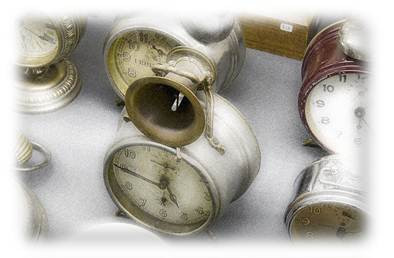
\includegraphics[height=4.5cm]{Snap.png}
\end{figure}
\vspace{2cm}}

\author{\textbf{Benötigte IDEs:}\\
\href{https://www.bluej.org/}{BlueJ}
\vspace{2cm}}

\date{\textbf{Verfasser:}\\
\href{https://nikothegreek.jimdofree.com/}{Niko Diamadis}\\
\vspace{0.5cm}
\textbf{Erstellungs-/ Änderungsdatum}\\
\today\enlargethispage{4cm}}
%----------------------------------------------------------------------------------------

%----------------------------------------------------------------------------------------
%   2. SEITE
%----------------------------------------------------------------------------------------
\doublespacing

\maketitle\thispagestyle{empty}

\numberwithin{equation}{section}
\cleardoublepage

\setcounter{page}{1}
\tableofcontents
%----------------------------------------------------------------------------------------


%----------------------------------------------------------------------------------------
%   3. UND NACHFOLGENDE SEITEN
%----------------------------------------------------------------------------------------
\newpage
\pagenumbering{arabic}  % Ändern der Seitenangabe

\cleardoublepage

\section{Timer im Codepad benutzen}

\subsection{Spielregeln \& Benutzung des Timers}

\begin{itemize}
    \barrow \textbf{1. Zeile}\\
    eine \texttt{Timer}-Variable \texttt{t} wird implementiert
    \barrow \textbf{2. Zeile}\\
    der Variable wird ein Objekt zugewiesen
    \barrow \textbf{3. Zeile}\\
    dem Integer \texttt{min} des Objekts \texttt{t} wird der Wert 2 zugewiesen
    \barrow \textbf{4. Zeile}\\
    dem Integer \texttt{max} des Objekts \texttt{t} wird der Wert 10 zugewiesen
    \barrow \textbf{5. Zeile}\\
    die Methode \texttt{starten} des Objekts \texttt{t} wird ohne Parameter aufgerufen
\end{itemize}

\subsection{'Testen'}

Zu dieser Aufgabe sind meines Erachtens nach keine Anleitungen und/oder Erläuterungen nötig.\\
Wenn doch Fragen aufkommen, schreib' einfach an \textbf{\href{mailto:nikodiamond3@gmail.com}{nikodiamond3@gmail.com}}.

\subsection{'Problemlösung'}

Die Methode funktioniert folgendermaßen:\\
Bei Aufruf der Methode werden als Parameter der minimale und der maximale Wert angegeben. Diese werden aber nur \texttt{min} und \texttt{max} zugewiesen, wenn \texttt{minimal} größer oder gleich 0 ist und wenn \texttt{maximal} kleiner oder gleich 0 ist.\\
Es ist jedoch immer noch möglich, die Attribute \texttt{min} und \texttt{max} über die Direkteingabe wieder zu verändern.

\newpage

\subsection{Privaten Zugriff}

Zu dieser Aufgabe sind meines Erachtens nach keine Anleitungen und/oder Erläuterungen nötig.\\
Wenn doch Fragen aufkommen, schreib' einfach an \textbf{\href{mailto:nikodiamond3@gmail.com}{nikodiamond3@gmail.com}}.

\newpage

\section{Fachkonzept - Kapselung}

Zu dieser Seite sind meines Erachtens nach keine Anleitungen und/oder Erläuterungen nötig.\\
Wenn doch Fragen aufkommen, schreib' einfach an \textbf{\href{mailto:nikodiamond3@gmail.com}{nikodiamond3@gmail.com}}.

\newpage

\section{Übungen}

\subsection{Geburtstagsschwindler}

\begin{figure}[!h]
	\centering
	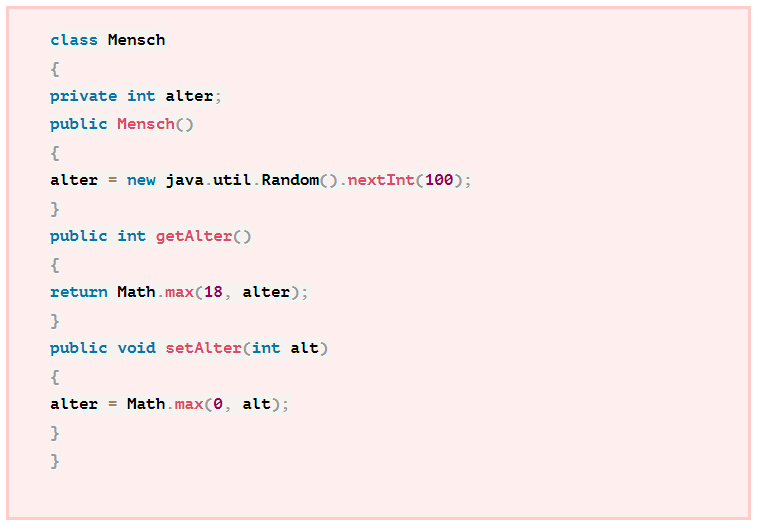
\includegraphics[height=9.5cm]{2.3.1.3/3.Uebungen/1-1.png}
\end{figure}

\subsection{private vs. public}

\begin{figure}[!h]
	\centering
	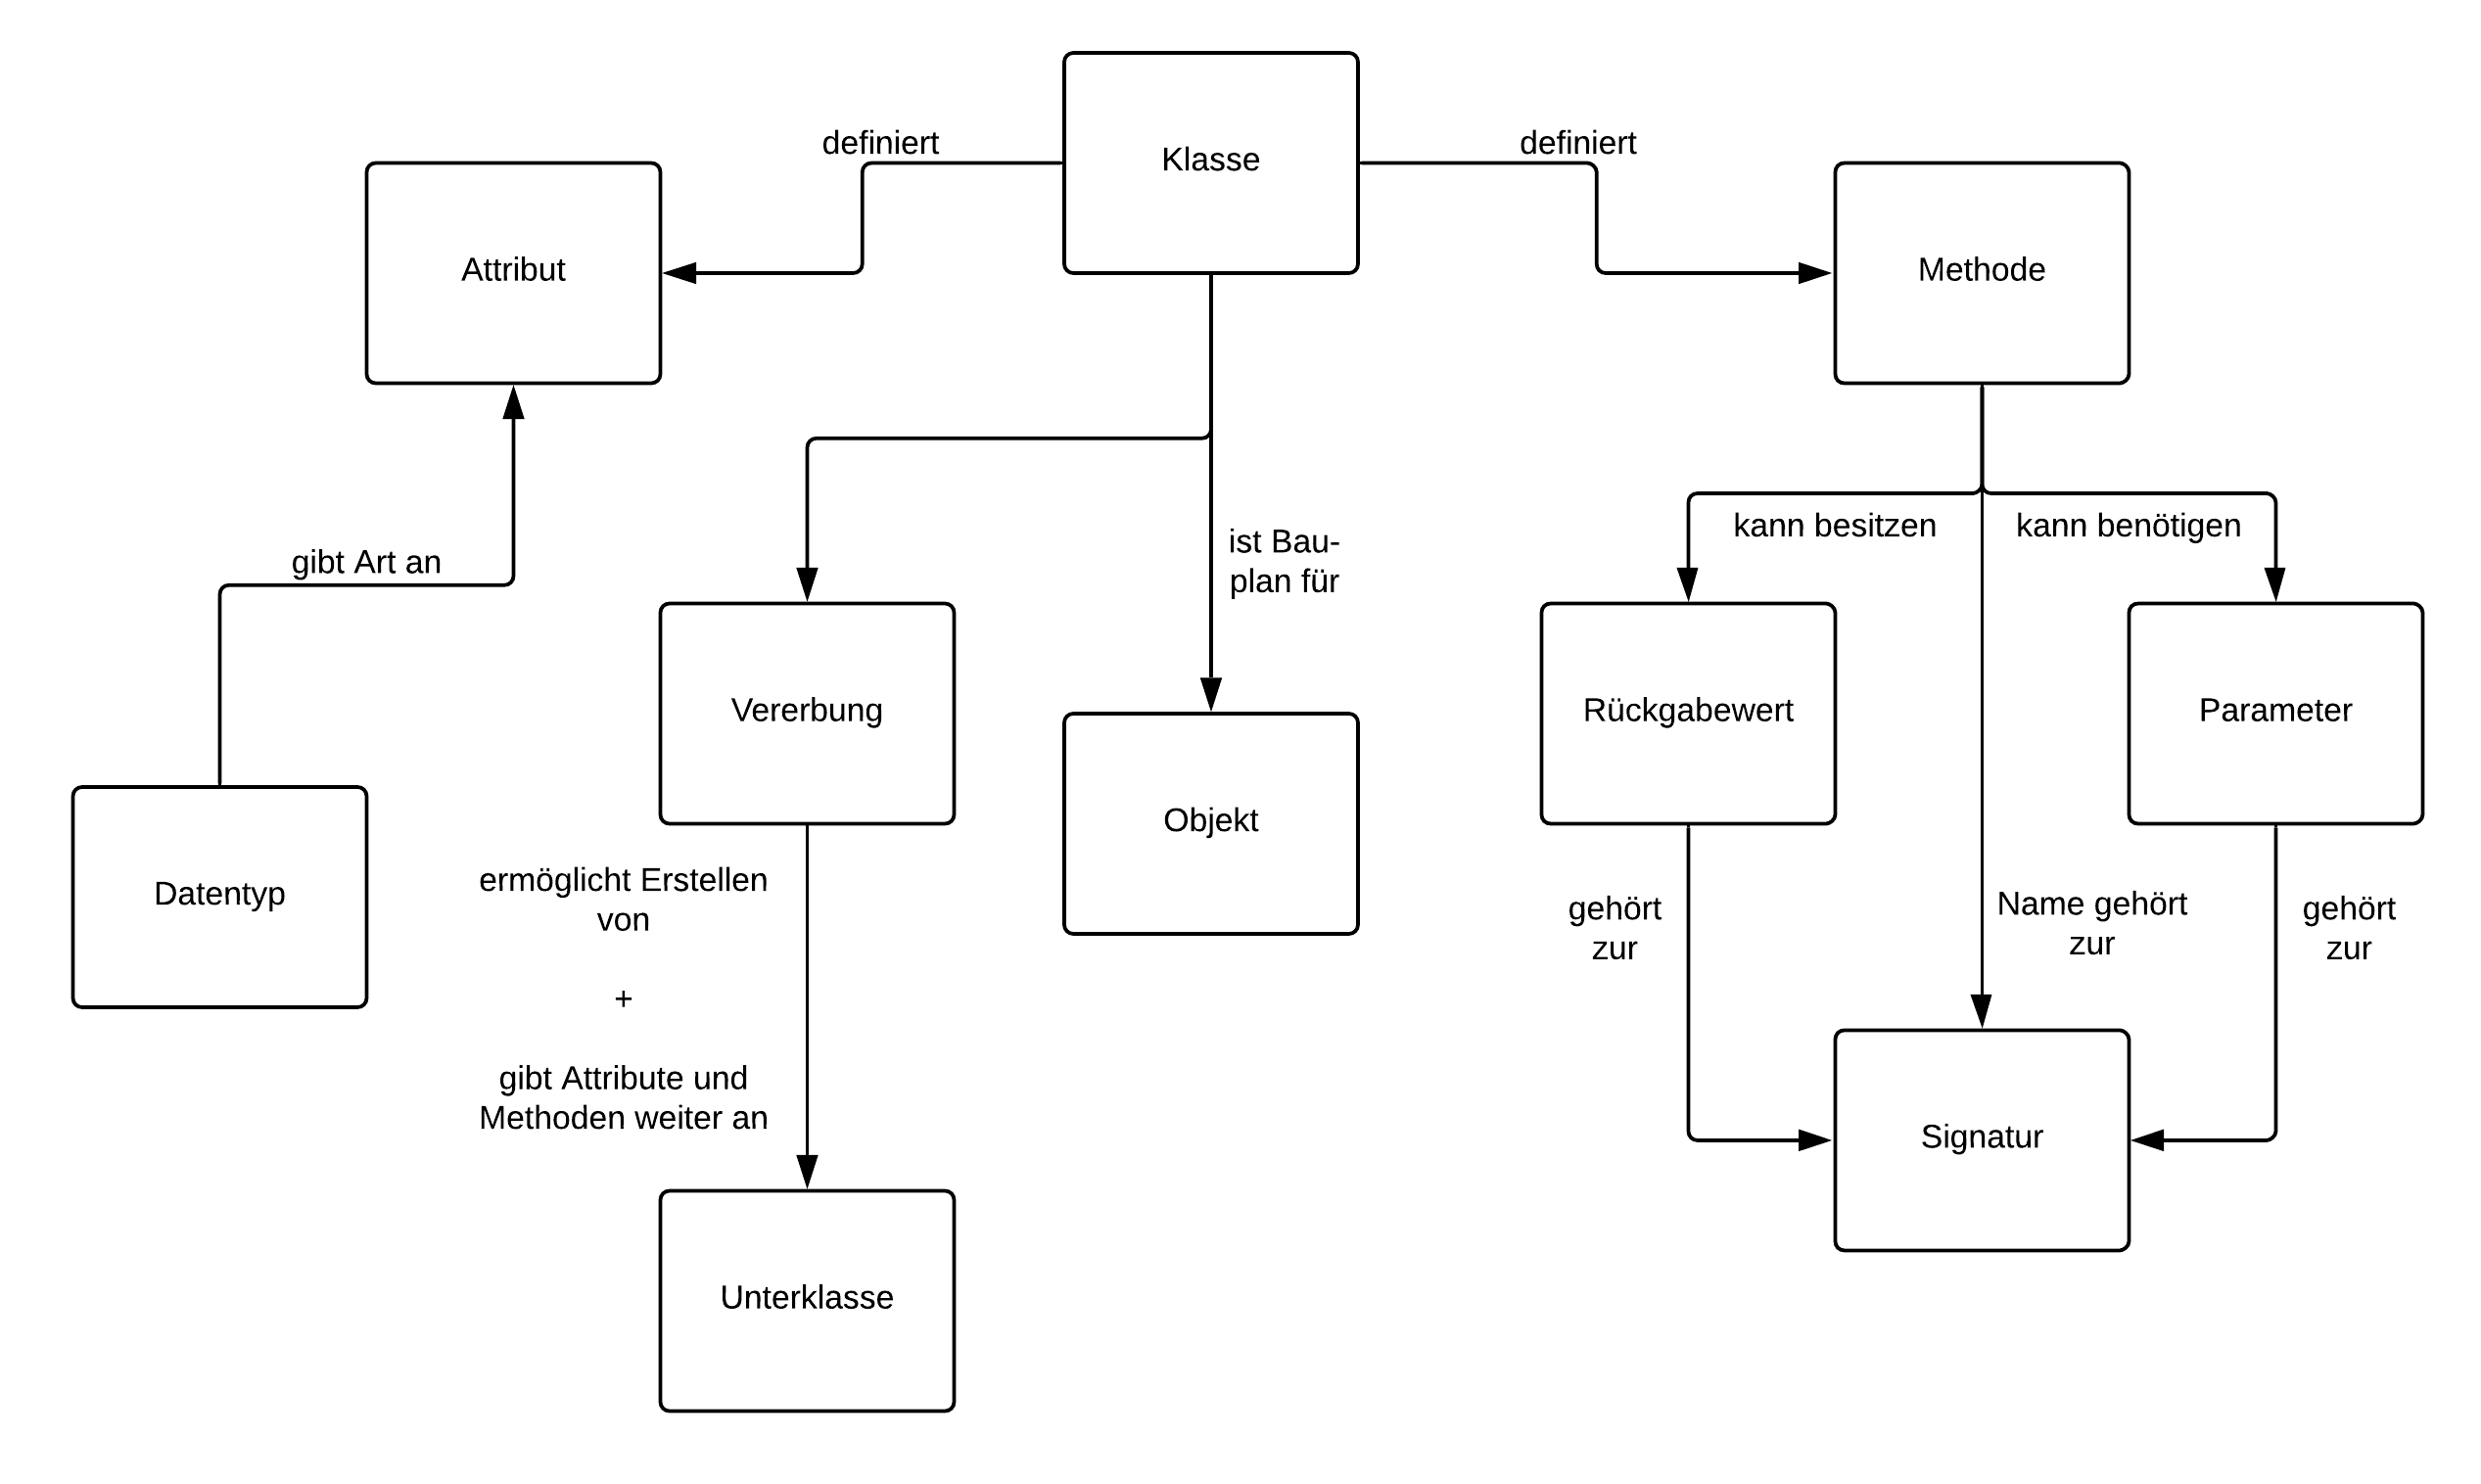
\includegraphics[height=5cm]{2.3.1.3/3.Uebungen/2-1.png}
\end{figure}

\newpage

\subsection{Stilfrage}

Dies ist eine gute Idee, da nur so sichergestellt werden kann, dass das Programm so wie geplant funktioniert. Eventuell sind es auch Daten, die die Nutzer nichts angeht oder womit sie womöglich nichts anfängen können.\\
Die Benutzung einer Klasse ändert sich durch Anpassen der Erreichbarkeit vonseiten des Nutzers dahingehend, dass alle Attribute privat sind und nur die Attribute, welche vom Nutzer geändert werden dürfen, von einer set-Methode beeinträchtigt werden.

\end{document}